\subsection{Разработка базы данных}
В процессе разработки программы для заполнения медицинской карты отделения неотложной медицинской помощи была разработана база данных на основе SQLite. База данных состоит из четырех основных таблиц: Users, Cards, FullCards и Catalogs. В данном подразделе будет подробно описана структура каждой из таблиц, а также основные связи между ними.

При разработке программы для работы с базой данных были реализованы различные функции, такие как добавление, редактирование и удаление записей, а также выполнение разнообразных запросов для поиска и фильтрации данных. Благодаря использованию SQLite в качестве хранилища данных, программа обеспечивает автономность и возможность работы без постоянного подключения к сети Интернет.

Взаимодействие с базой данных осуществляется через классы-репозитории, которые инкапсулируют логику работы с таблицами и предоставляют высокоуровневый интерфейс для взаимодействия с данными. Это позволяет упростить код программы и сделать его более удобным для дальнейшей поддержки и развития. ER диаграмма базы данных представлена на рисунке \ref{fig:figdb}.

\begin{figure}
  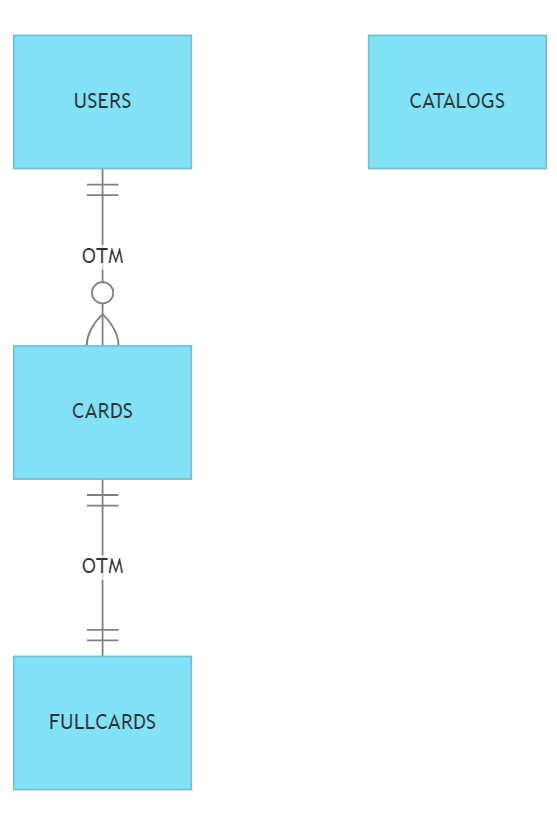
\includegraphics[scale=0.6]{inc/db.png}
  \caption{Диаграмма базы данных}
  \label{fig:figdb}
\end{figure}

\subsubsection{Таблица Users}

Таблица Users содержит информацию об авторизованных пользователях (врачах) и состоит из следующих полей:
\begin{itemize}
    \item id (INTEGER, PRIMARY KEY) - идентификатор пользователя;
    \item email (TEXT) - электронная почта пользователя. 
\end{itemize}

Для обеспечения быстрого поиска по электронной почте пользователей, поле email индексируется.

\subsubsection{Таблица Cards}

Таблица Cards представляет собой набор базовых сведений о медицинских картах. Структура таблицы включает следующие поля:
\begin{itemize}
    \item id (INTEGER, PRIMARY KEY) - идентификатор записи;
    \item id\_user (INTEGER) - идентификатор пользователя, создавшего медицинскую карту, являющийся внешним ключом, связанный с полем id таблицы Users;
    \item name (TEXT) - название медицинской карты;
    \item date (TEXT) - дата создания медицинской карты;
    \item type (TEXT) - тип медицинской карты (например, \enquote{готовая}, \enquote{архивная} и т. д.);
    \item comment (TEXT) - дополнительные комментарии к медицинской карте.
\end{itemize}

Между таблицами Users и Cards установлена связь \enquote{один ко многим}, так как один пользователь может создать несколько медицинских карт. А для обеспечения быстрого поиска дополнительно индексируются поля name, date и type дополнительно индексируются.

\subsubsection{Таблица FullCards}

Таблица FullCards содержит полную информацию о медицинских картах, включая все необходимые данные, заполненные врачом. Структура таблицы состоит из следующих полей:
\begin{itemize}
    \item id (INTEGER PRIMARY KEY) - идентификатор записи;
    \item id\_preview\_card (INTEGER) - идентификатор записи в таблице Cards, являющийся внешним ключом, связанный с полем id таблицы Cards;
    \item более 80 полей необходимых для заполнения медицинской карты. Поля могут содержать различные данные, такие как сведения о состоянии пациента, результаты анализов, диагнозы и т. д.
\end{itemize}

Между таблицами FullCards и Cards установлена связь \enquote{один к одному}, так как для каждой записи в таблице Cards существует только одна соответствующая запись в таблице FullCards, содержащая полную информацию о медицинской карте.

\subsubsection{Таблица Catalogs}

Таблица Catalogs представляет собой независимую структуру данных, которая не связана ни с одной другой таблицей. Она может содержать различные справочные данные, которые используются для обозначения или классификации информации в медицинской карте. Структура этой таблицы включает следующие поля:

\begin{itemize}
    \item id (INTEGER, PRIMARY KEY) - идентификатор записи, уникальное и автоматически генерируемое число;
    \item name (TEXT) - поле, содержащее название записи. Данное поле индексируется для обеспечения быстрого доступа и поиска по нему;
    \item text (TEXT) - поле, содержащее текст для записи.
\end{itemize}